\documentclass[11pt]{article}
\usepackage[T1]{fontenc}
\usepackage{lmodern}
\usepackage{amsmath,amssymb,amsthm}
\usepackage{mathtools}
\usepackage{geometry}
\geometry{margin=1in}
\usepackage{booktabs}
\usepackage{enumitem}
\usepackage{xcolor}
\usepackage{graphicx}
\usepackage{float}
\usepackage{caption}
\usepackage{microtype}
\usepackage{tikz}
\usetikzlibrary{calc,positioning,fit,shapes.geometric,arrows.meta}
\usepackage{hyperref}

\theoremstyle{plain}
\newtheorem{lem}{Lemma}

\theoremstyle{remark}
\newtheorem*{spinefact}{Spine fact}

\newtheoremstyle{modelclaim}
  {6pt plus 2pt minus 2pt}
  {6pt plus 2pt minus 2pt}
  {\normalfont}
  {}
  {\itshape}
  {.}
  {\newline}
  {\thmname{#1}\thmnote{ (#3)}}
\theoremstyle{modelclaim}
\newtheorem*{model}{Model}

% Upright O,C so Q_O cannot be read as Q\circ
\newcommand{\QO}{Q_{\mathrm{O}}}
\newcommand{\QC}{Q_{\mathrm{C}}}
\newcommand{\XO}{X_{\mathrm{O}}}
\newcommand{\sigZ}{\sigma(Z)}
\newcommand{\pPsi}{p(\Psi,t)}
\newcommand{\pq}{p(q,t)}
\newcommand{\Op}{O[\Psi]}
\newcommand{\piO}{\pi_{\mathrm{O}}}

\usepackage{microtype}
\usepackage{caption}
\usepackage{float}
\captionsetup{
  font=small,
  labelfont=bf,
  skip=6pt
}

\title{Helicoid--catenoid generators\\[2pt]
\large A companion note to QGA, labeled Model}
\author{Arena draft}
\date{Claim label: \textbf{Model} --- not a theorem of the QGA spine}

\begin{document}
\maketitle
\vspace{-1.0em}

\begin{abstract}
\noindent
The mix \(Q=\QO+\sigma(Z)\,\QC\) is a mass-preserving forward operator
for a split: life versus catalog.
It is a \textbf{Model}, not a theorem, and not part of the Hatcher lift.
QGA's spine remains quaternion orders, Hopf, and topographs.
This note defines four words operationally,
proves the cheap lemmas,
says what the Hopf fiber adds,
and states one \(\sigma\)-sweep protocol.
\end{abstract}

\section*{Scope}

This is a companion note, not a chapter of QGA.
The book's spine is quaternion orders, Hopf, and topographs
(\url{https://github.com/kinaar8340/qga}).
The mix
\[
Q = \QO + \sigma(Z)\,\QC
\]
is a different object: a labeled \textbf{Model} of incompleteness dynamics.
It is not a theorem about number theory, and it is not part of the Hatcher lift.

Spine facts used as input remain the only theorems in scope:
\(S^{3}\subset\mathbb{H}\),
\(h:S^{3}\to S^{2}\),
\(N(q)=q\bar q=1\).
Observational numerology (\(350/\pi\), Magic Islands, pulsar coincidences)
is out of this note.

Ranked roles are not used here.
They are not defined operationally in the generator, so they are dropped.
No equation for \(Z\) appears in this note.

\section{Four words, operationally}
\label{sec:words}

Four loaded words. Each is a map or a functional of the density \(p\),
not a metaphor.

\paragraph{Life.}
Continuous transport.
\[
\QO\,p
:= -\nabla\cdot(\Op\,p)
\qquad\text{or, on \(S^{3}\),}\qquad
\QO\,p
:= -\operatorname{div}_{S^{3}}(\XO\,p).
\]
\(\sigma=0\) is pure life: \(\partial p/\partial t = \QO\,p\).

\paragraph{Catalog.}
Jump kernel, already written as gain minus loss.
\[
\QC\,p
:= \int\bigl[w(\Psi\mid\Psi')p(\Psi')
      -w(\Psi'\mid\Psi)p(\Psi)\bigr]\,d\Psi'
\]
or the lattice sum on \(\Lambda\).
No extra minus is placed on this lobe.

\paragraph{Correction.}
A map from an error signal into the gate or the kernel.
Write \(e = A[p]-A^{\ast}\).
Correction is a (possibly set-valued) map
\[
C:\ (p,e)\ \mapsto\ \bigl(\sigma',\,w'\bigr)
\]
that changes \(\sigma(Z)\) or \(w\), and nothing else.
If \(C\) is absent, \(\sigma\) is an exogenous schedule.
Protocol~S1 does not use \(C\).

\paragraph{Alignment.}
A stated functional \(A[p]\in\mathbb{R}\) of the density.
Correction is defined only relative to a named \(A\).
This note does not promote a unique \(A\);
a protocol run must name one before it reports.
Life-drift \(D(\sigma,t)=\mathrm{KL}(p_{t}^{\sigma}\Vert p_{t}^{0})\)
is a different functional; it is not \(A\).

The lens of the Venn is \(\partial p/\partial t\), never a third operator.
The slogan ``the catalog cannot prove it captured the life''
is Lemmas~\ref{lem:mass}--\ref{lem:markov} and the Spine fact (Hopf remainder).

\section*{Shared notation}
\begin{center}
\begin{tabular}{@{}ll@{}}
\toprule
Symbol & Meaning \\
\midrule
$\QO\,p$ & life: $-\nabla\cdot(\Op\,p)$ or $-\operatorname{div}_{S^{3}}(\XO\,p)$ \\
$\QC\,p$ & catalog / jump kernel (gain$-$loss already inside) \\
$\Op$ & vector field on generic $\Psi$ (not the configuration manifold) \\
$\XO$ & $\XO(q)=iq$, right-invariant fiber field of $h$ \\
$h$ & Hopf map $S^{3}\to S^{2}$ (catalog projection; QGA's one map) \\
$\sigZ$ & catalog gate ($\sigma=0$: pure life) \\
$Z$ & coarse parameter (Scope: no equation for $Z$) \\
$Q=\QO+\sigZ\,\QC$ & master operator (plus, always) \\
$r(\sigma,t)$ & $\displaystyle\frac{\lVert\sigma\,\QC p\rVert_{1}}{\lVert\QO p\rVert_{1}+\varepsilon}$ \\
$D(\sigma,t)$ & life-drift $\mathrm{KL}(p_{t}^{\sigma}\Vert p_{t}^{0})$ \\
$A[p]$ & alignment, a named functional of $p$ \\
$C$ & correction, a map $(p,e)\mapsto(\sigma',w')$ \\
\bottomrule
\end{tabular}
\end{center}

\section{Formal full object}

\begin{model}[Helicoid--catenoid master equation]
Mass-preserving forward operator on a configuration density.
Scope: labeled Model, not a theorem of QGA.
\end{model}

\paragraph{Definitions.}
\begin{align}
\QO\,p
&:= -\nabla\cdot(\Op\,p),
\label{eq:formal-QO}\\
\QC\,p
&:= \int\bigl[w(\Psi\mid\Psi')p(\Psi')
      -w(\Psi'\mid\Psi)p(\Psi)\bigr]\,d\Psi',
\label{eq:formal-QC}\\
\frac{\partial p(\Psi,t)}{\partial t}
&= Qp
= \QO\,p + \sigma(Z)\,\QC\,p.
\label{eq:formal-master}
\end{align}

\paragraph{Pictures, not the manifold.}
The helicoid and catenoid in Figure~\ref{fig:formal}\ illustrate the split:
continuous transport versus catalog jumps.
They are not the configuration manifold.
Equations~\eqref{eq:formal-QO}--\eqref{eq:formal-master} are written on a
generic \(\Psi\)-space with a vector field and a kernel.

\paragraph{Standing hypotheses.}
\(\Op\) is \(C^{1}\) with at most linear growth (or no flux at infinity).
When the configuration space is \(S^{3}\), the field is \(\XO(q)=iq\),
tangent to \(S^{3}\).
\(w\ge 0\) is measurable, and the outgoing rate is finite:
\(\int w(\Psi'\mid\Psi)\,d\Psi'<\infty\) for a.e.\ \(\Psi\).
\(Z\) is coarse: \(\sigma(Z)\) is a parameter of the fast operator (Scope).
\(p(\,\cdot\,,t)\) is a probability density.

\paragraph{Symbols.}
\begin{itemize}[leftmargin=1.4em,itemsep=2pt,topsep=4pt,parsep=0pt]
  \item \(\Psi\): state variable on a generic configuration space.
  \item \(p(\Psi,t)\): density.
  \item \(\Op\): vector field (life). The helicoid is a picture of this split,
        not the manifold of \(\Psi\).
  \item \(w(\Psi\mid\Psi')\ge 0\): transition kernel (catalog).
  \item \(\sigma(Z)\ge 0\): catalog gate (\(\sigma=0\) is pure life).
\end{itemize}

\paragraph{Orientation.}
Upper exclusive: \(\QO\,p\) (life).
Lens: \(\partial p/\partial t\).
Lower exclusive: \(\sigma(Z)\,\QC\,p\) (catalog).

\begin{center}
\textit{The catalog needs the life; the life is not the catalog.}
\end{center}

\begin{figure}[H]
  \centering
  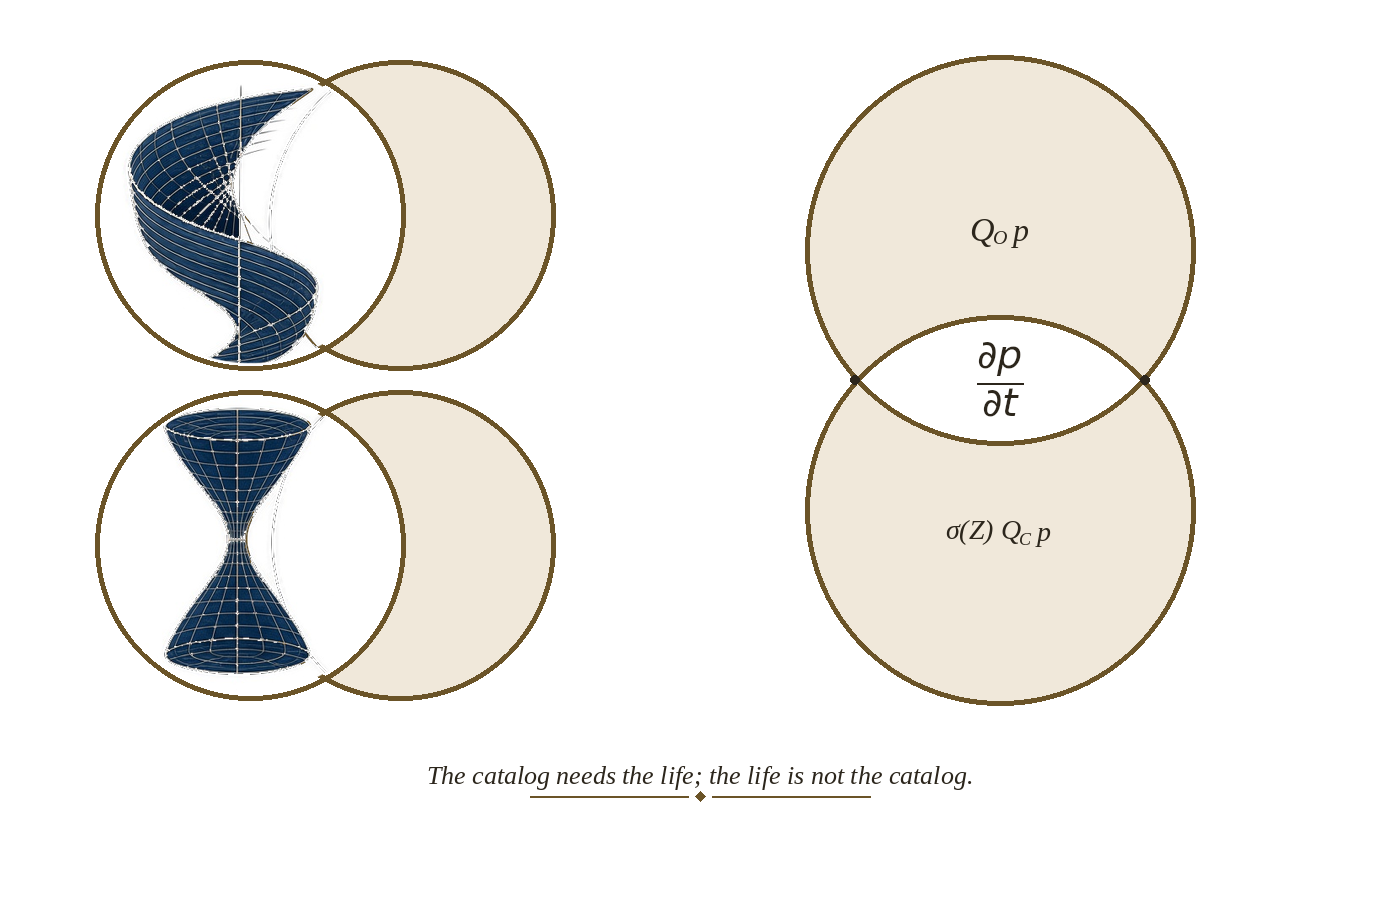
\includegraphics[width=0.88\linewidth]{../fig/formal-full-object.png}
  \caption{Formal full object.
  Life transport \(\QO\) on the helicoid lobe;
  catalog jumps \(\sigma(Z)\,\QC\) on the catenoid lobe;
  the observed motion \(\partial p/\partial t\) only in the lens.
  Surfaces illustrate the split; they are not the configuration manifold.}
  \label{fig:formal}
\end{figure}

\section{Cheap lemmas}
\label{sec:lemmas}

These two lemmas are internal to the Model.
The Hopf remainder is a spine fact, not a lemma about \(Q\).

\begin{lem}[Mass]
\label{lem:mass}
Under the standing hypotheses,
\[
\int \QO\,p\,d\Psi = 0,
\qquad
\int \QC\,p\,d\Psi = 0,
\qquad
\int Qp\,d\Psi = 0.
\]
\end{lem}

\begin{proof}
By definition \(\QO\,p=-\nabla\cdot(\Op\,p)\).
The divergence theorem (no flux at infinity) gives
\(\int\nabla\cdot(\Op\,p)\,d\Psi=0\), hence \(\int \QO\,p\,d\Psi=0\).
For the kernel, Fubini and the change of names \((\Psi,\Psi')\mapsto(\Psi',\Psi)\)
cancel the two terms of~\eqref{eq:formal-QC}, hence \(\int \QC\,p\,d\Psi=0\).
Because \(Z\) is coarse, \(\sigma(Z)\) is a parameter of the fast operator, so
\(\int\sigma(Z)\,\QC\,p\,d\Psi=\sigma(Z)\int \QC\,p\,d\Psi=0\).
The third claim is the sum.
\end{proof}

\begin{lem}[Markov]
\label{lem:markov}
Under the standing hypotheses, \(Q^{\ast}1=0\).
The jump piece \(\sigma(Z)\,\QC\) is a Kolmogorov forward operator:
\(w\ge 0\) and \(\sigma(Z)\ge 0\).
Mass preservation is Lemma~\ref{lem:mass}.
Existence of the semigroup is not claimed.
\end{lem}

\begin{proof}
Lemma~\ref{lem:mass} says \(\int Qp\,d\Psi=0\) for every density \(p\),
which is the dual condition \(Q^{\ast}1=0\).
The kernel \(w\ge 0\) makes \(\QC\) the forward operator of a jump process;
\(\sigma(Z)\ge 0\) scales that operator and does not flip its sign.
The vector-field piece is Liouville transport.
The sum is with \(+\) (never an extra minus on \(\QC\)).
No third lobe.
\end{proof}

\begin{spinefact}[Hopf remainder]
\label{sf:hopf}
Spine input, not a lemma about \(Q\), not proved here:
\(h:S^{3}\to S^{2}\) is a locally trivial \(S^{1}\)-bundle and is not
globally trivial.
Any catalog observable that factors through \(h\) cannot invert the fiber
coordinate.
Locally, on a trivialization \(U\times S^{1}\), the two generators of the
Model may share the bundle metric.
Globally they do not coincide, and the catalog cannot prove it has captured
the life.
\end{spinefact}

Local triviality of \(h\) is the local metric agreement.
Equivalently, \(h\) has no global section:
the fiber \(S^{1}\) is the life the base does not see
(\(\pi_{1}(S^{3})=0\) while \(\pi_{1}(S^{2}\times S^{1})\cong\mathbb{Z}\)
already forbids a product).
The Model uses that fact as input; it does not become a number-theory theorem
by being written next to Hopf.

\section{What the quaternionic lift adds}

The \(3\)-D helicoid--catenoid picture already carries the incompleteness
slogan (Figure~\ref{fig:formal}).
The Hopf version is worth writing only if the fiber is used.

\paragraph{Diagram, not extra symbols.}
Base \(S^{2}\) is catalog-visible.
Fiber \(S^{1}\) is the remainder.
The map \(h\) is the catalog projection.

\begin{center}
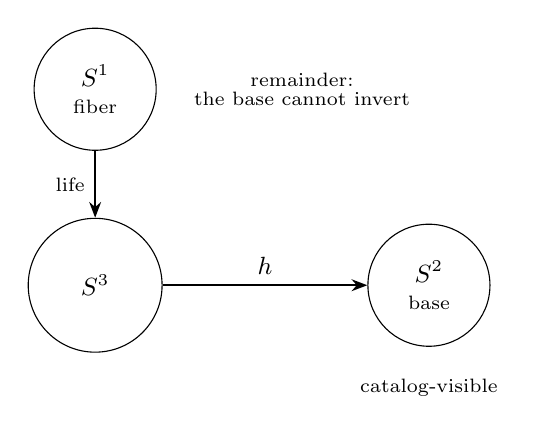
\begin{tikzpicture}[
  font=\small,
  every node/.style={align=center},
  arr/.style={-{Stealth[length=2mm]}, thick}
]
  \node[draw, circle, minimum size=1.55cm] (s1) {\(S^{1}\)\\[-1pt]\scriptsize fiber};
  \node[draw, circle, minimum size=1.7cm, below=0.85cm of s1] (s3) {\(S^{3}\)};
  \node[draw, circle, minimum size=1.55cm, right=2.6cm of s3] (s2) {\(S^{2}\)\\[-1pt]\scriptsize base};
  \draw[arr] (s1) -- node[left, font=\scriptsize] {life} (s3);
  \draw[arr] (s3) -- node[above] {\(h\)} (s2);
  \node[font=\scriptsize, below=0.28cm of s2] {catalog-visible};
  \node[font=\scriptsize, right=0.15cm of s1, xshift=0.2cm] {remainder:\\[-1pt]the base cannot invert};
\end{tikzpicture}
\end{center}

\begin{model}[Hopf lift of the helicoid--catenoid generator]
Same split, different stage.
Dynamics on \(S^{3}\) and on the gauged Hopf lattice.
Spine input only:
\(S^{3}\subset\mathbb{H}\),
\(h:S^{3}\to S^{2}\),
\(N(q)=q\bar q\).
See \url{https://github.com/kinaar8340/qga}.
\end{model}

\paragraph{Definitions.}
\begin{align}
\XO(q)
&= iq,
\label{eq:qga-XO}\\
\QO\,p
&:= -\operatorname{div}_{S^{3}}(\XO\,p),
\label{eq:qga-QO}\\
\QC\,p
&:= \sum_{q'\sim q}
      \bigl[w(q\mid q')p(q')-w(q'\mid q)p(q)\bigr],
\label{eq:qga-QC}\\
\frac{\partial p(q,t)}{\partial t}
&= Qp
= \QO\,p + \sigma(Z)\,\QC\,p.
\label{eq:qga-master}
\end{align}
Here \(q'\sim q\) means neighbors in the gauged Hopf lattice
(or topograph edges).
That \(\sim\)\, is QGA Open Problem~1:
the kernel \(w\) is exogenous.
It is not claimed to be Hatcher's Farey lift.

Life on this stage is transport along the structure-group fiber of
QGA's \(h\): left common-phase \(q\mapsto e^{i\theta}q\), generated by
the right-invariant field~\eqref{eq:qga-XO}.
The left-invariant field \(q\mapsto qi\) generates the fiber of the other
Hopf map \(q\mapsto qi\bar q\) and is not used.
No extra invariance claim is a term in \(Q\).

Mass conservation is Lemma~\ref{lem:mass} with \(d\Psi\) replaced by
the Riemannian measure \(d\mu\) on \(S^{3}\).
Markov is Lemma~\ref{lem:markov}: \(Q^{\ast}1=0\), and the jump piece
is Kolmogorov forward.
The remainder is the Spine fact (Hopf remainder).
\(N(q)=1\) is the standing constraint on this stage.
Linking of fibers is a property of \(h\), not something the ODE proves.

\paragraph{Symbols.}
\begin{itemize}[leftmargin=1.4em,itemsep=2pt,topsep=4pt,parsep=0pt]
  \item \(q\in S^{3}\subset\mathbb{H}\),
        \(h:S^{3}\to S^{2}\),
        \(N(q)=q\bar q=1\).
  \item \(\XO(q)=iq\): right-invariant fiber field of \(h\) (life).
  \item \(w(q\mid q')\ge 0\): gauge / adjacency kernel on \(\Lambda\).
  \item \(\sigma(Z)\ge 0\): catalog gate (\(\sigma=0\): pure fiber life).
\end{itemize}

\begin{center}
\textit{The catalog needs the life; the life is not the catalog.}
\end{center}

\begin{figure}[H]
  \centering
  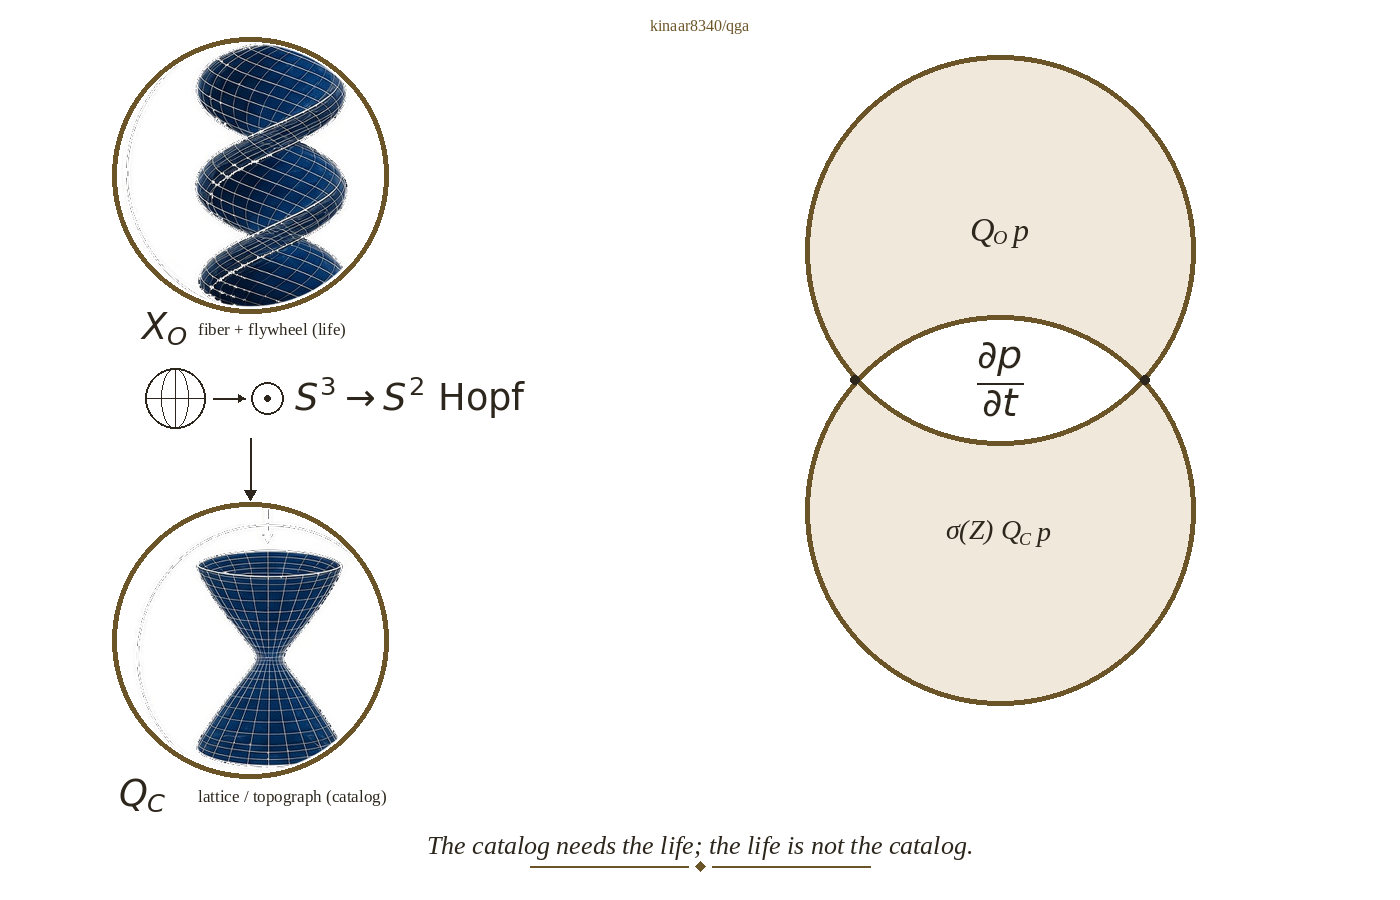
\includegraphics[width=0.88\linewidth]{../fig/qga-full-object.png}
  \caption{QGA full object, still a Model.
  \(\XO\) runs on the fiber;
  \(\QC\) runs on lattice / topograph edges;
  \(h:S^{3}\to S^{2}\) is the catalog projection that cannot invert the fiber.}
  \label{fig:qga}
\end{figure}

\paragraph{Comparison.}
\(\QO\) is advection in both objects (vector field on \(\Psi\),
fiber field on \(S^{3}\)).
\(\QC\) is the jump catalog in both (integral kernel, then lattice sum).
The lift changes the \emph{stage}
(\(S^{3}\), Hopf fiber, Hopf linking as a property of \(h\)),
not the \emph{split}.

\section{One simulation protocol}
\label{sec:protocol}

Without a sweep, ``without correction, adaptation takes control'' is a motto.
Protocol~S1 makes the motto a report.

S1 is open-loop.
Correction \(C\) is defined in \S\ref{sec:words} and unused here.
Protocol~S2 is the closed loop that feeds \(e=A[p]-A^{\ast}\) into \(\sigma\) or \(w\);
it is named so it cannot be smuggled into S1, and it is not run here.

\paragraph{Protocol S1 (\(\sigma\)-sweep).}
Freeze \(\Op\) (or \(\XO\)) and \(w\).
Fix an initial density \(p(\,\cdot\,,0)\) and a horizon \(T>0\).
Name an alignment functional \(A[p]\) before the run.
\(Z\) is frozen (Scope).

For a grid \(0=\sigma_{0}<\sigma_{1}<\cdots<\sigma_{N}\),
evolve
\[
\partial_{t}p = \QO\,p + \sigma\,\QC\,p
\]
and record, at \(t=T\):

\begin{center}
\begin{tabular}{@{}ll@{}}
\toprule
Report & Meaning \\
\midrule
dominance \(r(\sigma,t)\) &
  \(\displaystyle\frac{\lVert\sigma\,\QC p\rVert_{1}}{\lVert\QO p\rVert_{1}+\varepsilon}\) \\
life-drift \(D(\sigma,t)\) &
  \(\mathrm{KL}\bigl(p_{t}^{\sigma}\big\Vert p_{t}^{0}\bigr)\) \\
alignment \(A[p_{t}^{\sigma}]\) &
  named before the run \\
mixing time \(t_{\mathrm{mix}}(\sigma)\) &
  empirical time of the jump part to a fixed TV tolerance \\
attractor capture &
  mass of \(p\) on a named catalog-visible set \\
\bottomrule
\end{tabular}
\end{center}

Life-drift \(D\) and alignment \(A\) are different functionals.
This note's S1 plot names
\(A[p]=\mathrm{KL}(p\Vert\piO)\) with \(\piO\) a \(\sigma=0\) invariant
(the uniform measure on the circle).
That \(A\) tracks distance to uniform, not restoration of the life shape.
It does not promote that choice of \(A\) as unique.

Declare
\[
\sigma_{\ast}
:= \inf\bigl\{\sigma:\ r(\sigma,T)\ge 1\bigr\}
\]
the gate at which the jump term dominates the vector field at horizon \(T\).

\begin{figure}[H]
  \centering
  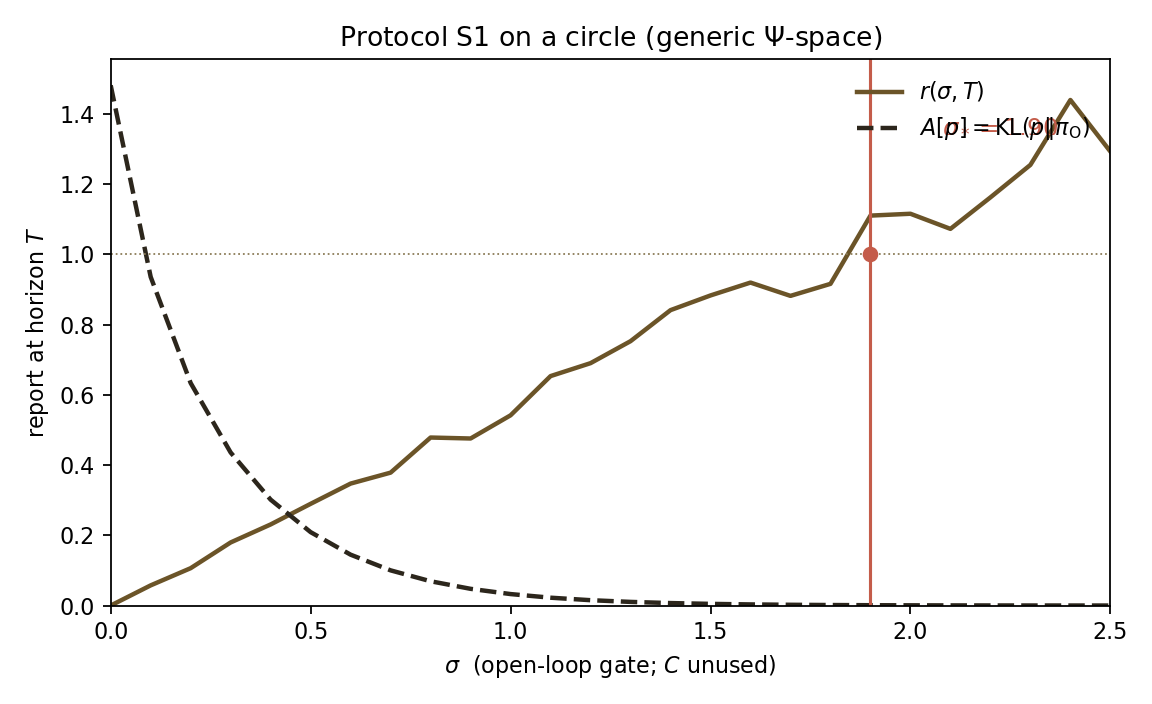
\includegraphics[width=0.88\linewidth]{../fig/s1-sweep.png}
  \caption{Protocol~S1, open-loop. Illustrative, not a lab figure of the Hopf stage.
  Space: the circle \(\mathbb{R}/(2\pi\mathbb{Z})\) (\(N=256\)).
  \(O=\partial_{\theta}\) (speed \(1\));
  \(\QC p=\piO-p\) with \(\piO\equiv 1/(2\pi)\)
  (rank-one jump to uniform, rate \(1\));
  \(T=2\), \(\varepsilon=10^{-12}\);
  initial \(p(\cdot,0)\) a bump at \(\pi\).
  Named alignment for this run:
  \(A[p]=\mathrm{KL}(p\Vert\piO)\) with \(\piO\) uniform.
  Life-drift \(D(\sigma,T)\) is not plotted; \(r(\sigma,T)\) and \(A[p]\) are.
  \(\sigma=0\) is pure transport; \(\sigma_{\ast}\) is where catalog jumps dominate.
  \(C\) is unused.}
  \label{fig:s1}
\end{figure}

\paragraph{Reading.}
Because S1 is open-loop, \(\sigma\) is the sweep parameter.
Jumps dominate when \(r(\sigma,T)\ge 1\).
Life-drift \(D(\sigma,T)=\mathrm{KL}(p_{T}^{\sigma}\Vert p_{T}^{0})\) grows.
The named \(A[p]=\mathrm{KL}(p\Vert\piO)\) drops because the catalog mixes
toward uniform.
This \(A\) is distance to the mixed state, not a target that restores the life shape.
A run that retunes \(\Op\), writes an equation for \(Z\),
or invents a third operator is not this protocol.

\paragraph{Out of scope.}
No \(350/\pi\), no Magic Islands, no pulsar coincidences,
no diffusion term, no Riemann examples.
Protocol~S2 is named above and not run.


\end{document}
